\documentclass[11pt]{article}
\usepackage[paperwidth=8.5in,paperheight=8.5in,margin=0.5in]{geometry}  % Square format
\usepackage{graphicx}
\usepackage{amsmath}
\usepackage{amssymb}
\usepackage{multicol}
\usepackage{tikz}

\pagestyle{empty}  % No page numbers

\title{\Huge\textbf{The Exceptional Bestiary}\\[0.3cm]
\large A Complete Atlas of Unique Root Systems}
\author{}
\date{}

\begin{document}

\maketitle

\begin{center}
\large\textit{``And the serpent swallowed the world, and in its belly lived 112 smaller serpents...''}
\end{center}

\vspace{1cm}

%% PAGE 1: THE FIVE EXCEPTIONAL PRIMES
\section*{I. The Five Exceptional Primes}

\begin{center}
\begin{tabular}{cc}
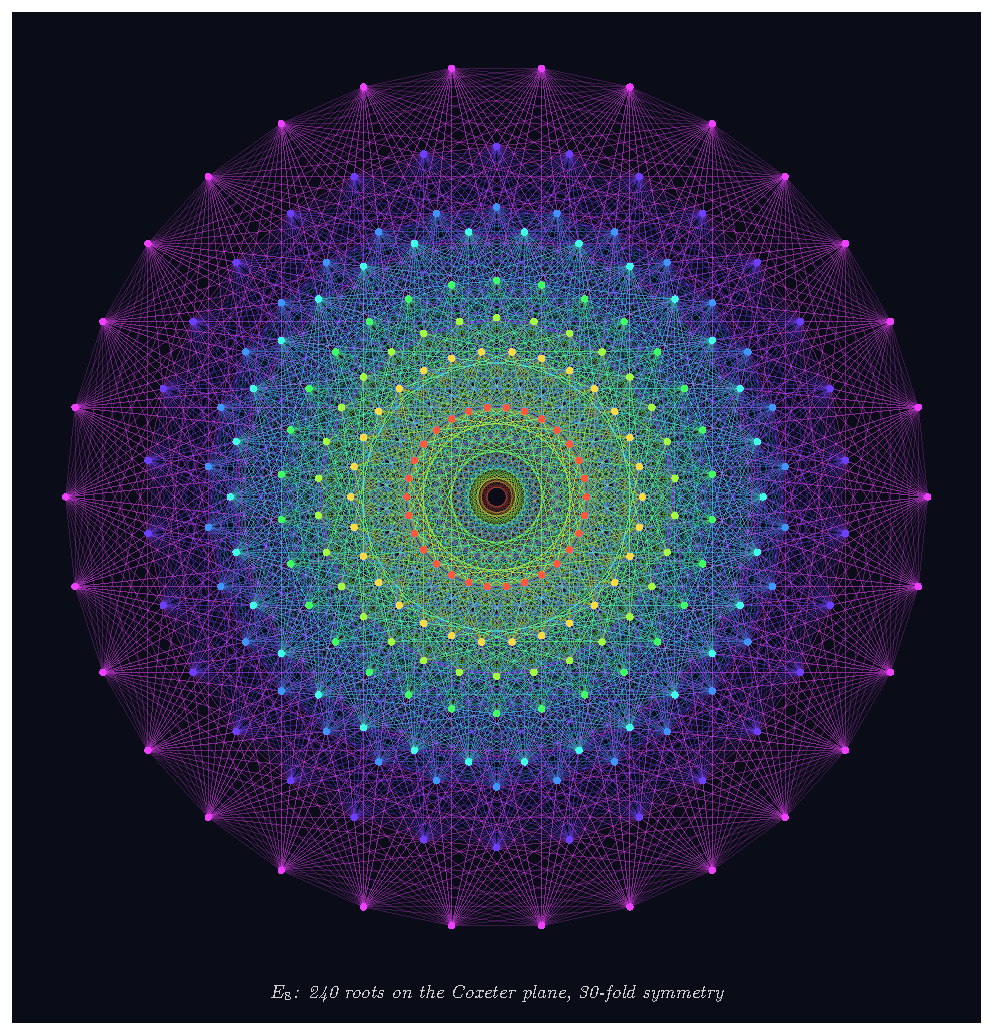
\includegraphics[width=0.4\textwidth]{e8_mandala.pdf} &
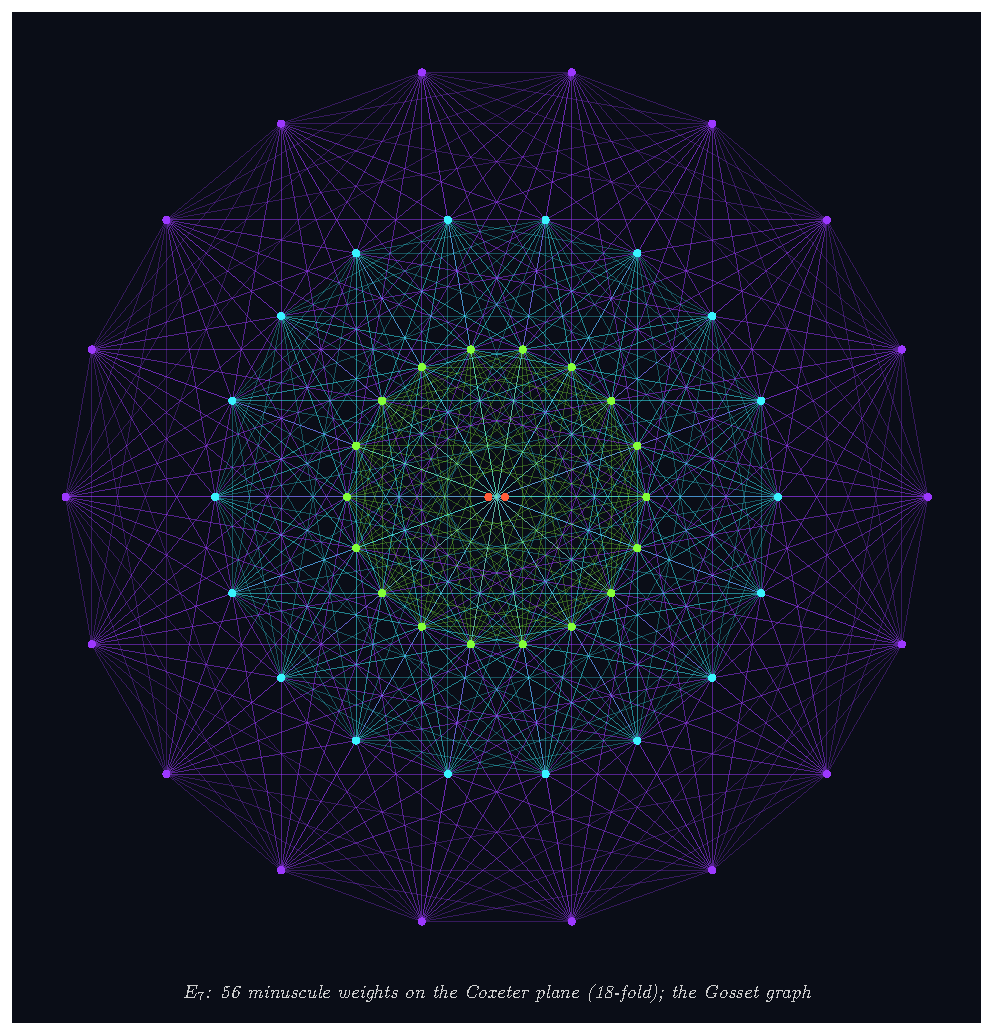
\includegraphics[width=0.4\textwidth]{e7_mandala.pdf} \\[0.2cm]
\textbf{E8: The Ouroboros} & \textbf{E7: The Sacred Cow} \\
240 roots, 30-fold & 56 weights, 18-fold \\[0.8cm]

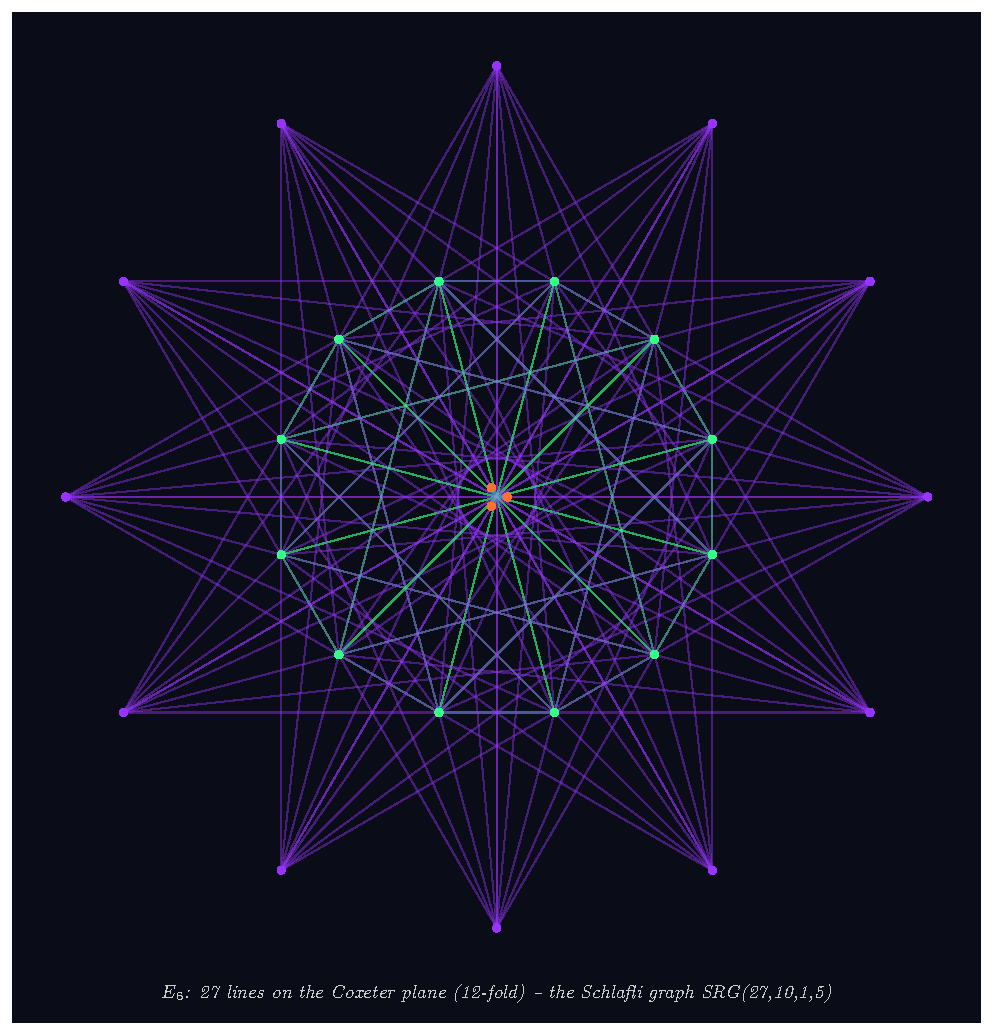
\includegraphics[width=0.4\textwidth]{e6_schlafli.pdf} &
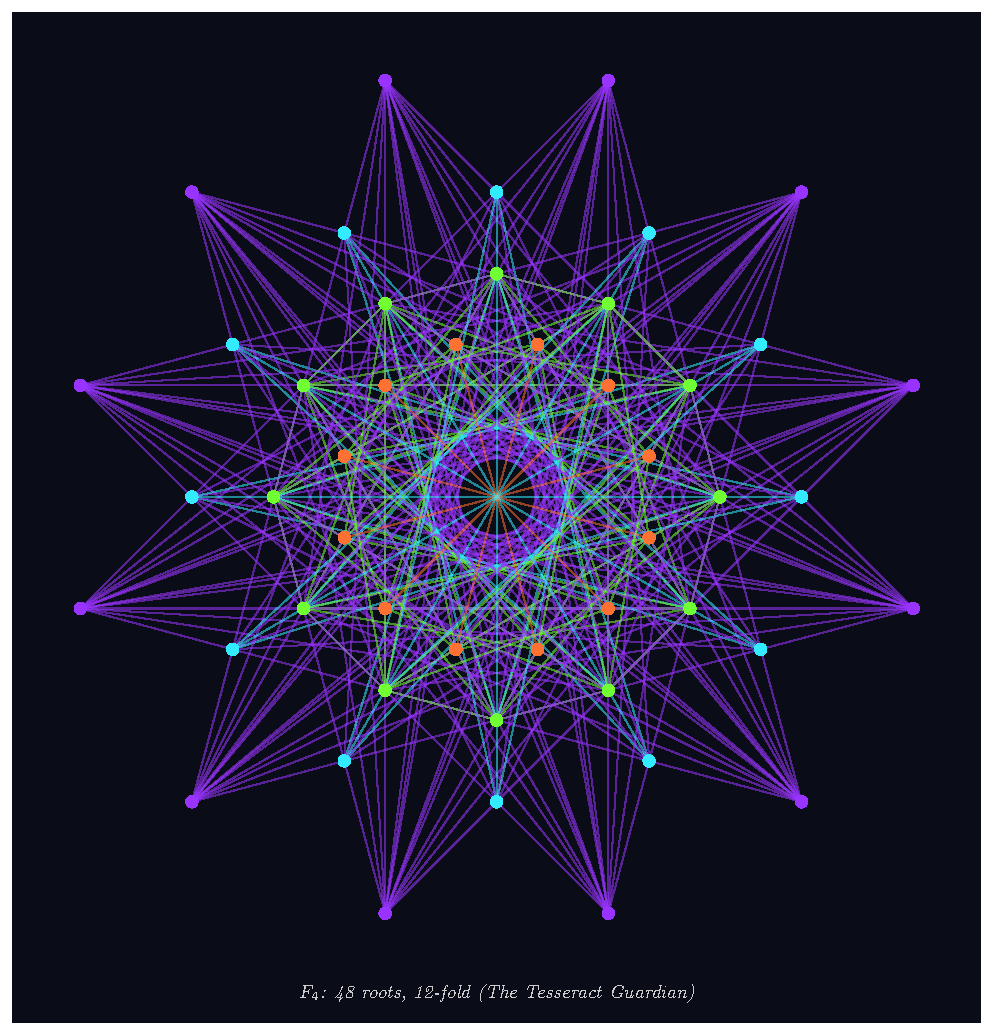
\includegraphics[width=0.4\textwidth]{f4_roots.pdf} \\[0.2cm]
\textbf{E6: The Trinity} & \textbf{F4: The Tesseract Guardian} \\
27 lines, 12-fold & 48 roots, 12-fold \\[0.8cm]

\multicolumn{2}{c}{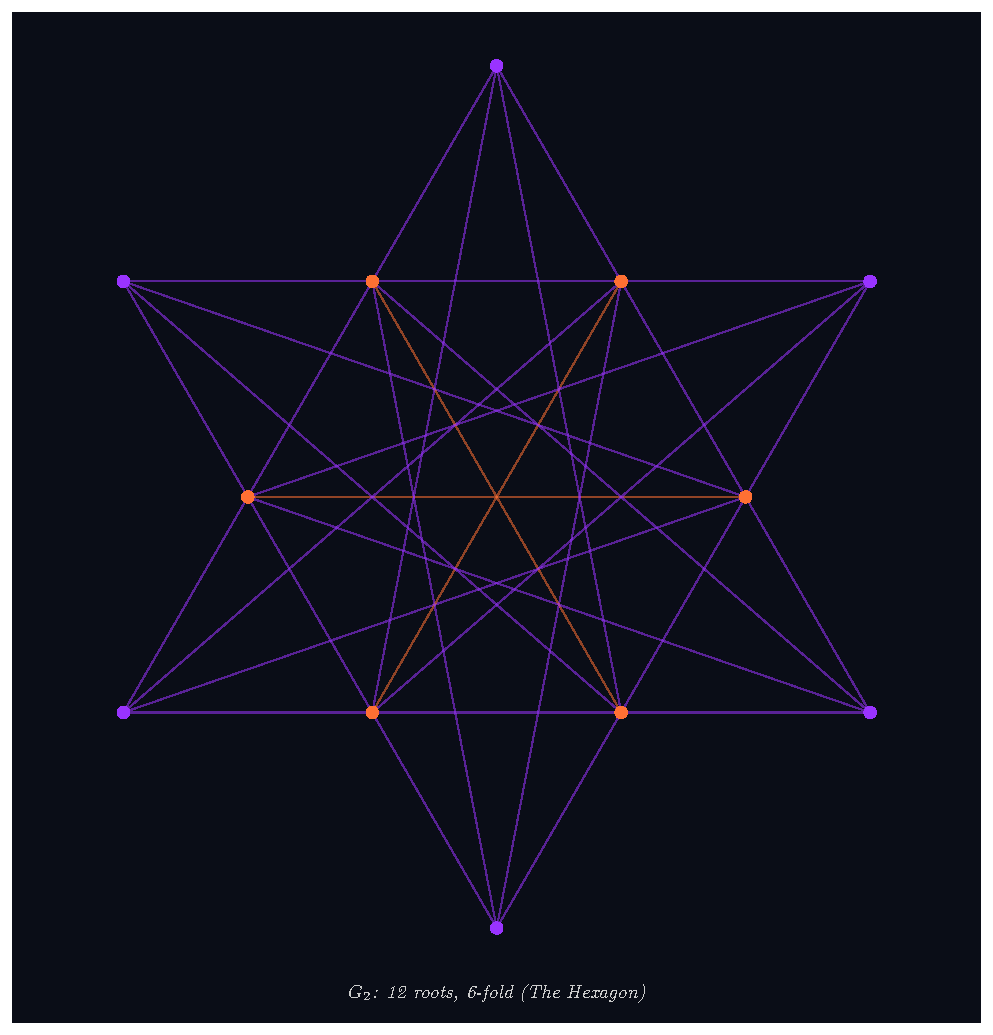
\includegraphics[width=0.4\textwidth]{g2_roots.pdf}} \\[0.2cm]
\multicolumn{2}{c}{\textbf{G2: The Hexagon / The Primal Inchworm}} \\
\multicolumn{2}{c}{12 roots, 6-fold} \\
\end{tabular}
\end{center}

\clearpage

%% PAGE 2: THE CLASSICAL SERIES
\section*{II. The Classical Series}

\subsection*{The D-Series (Demihypercubes)}

\begin{center}
\begin{tabular}{cc}
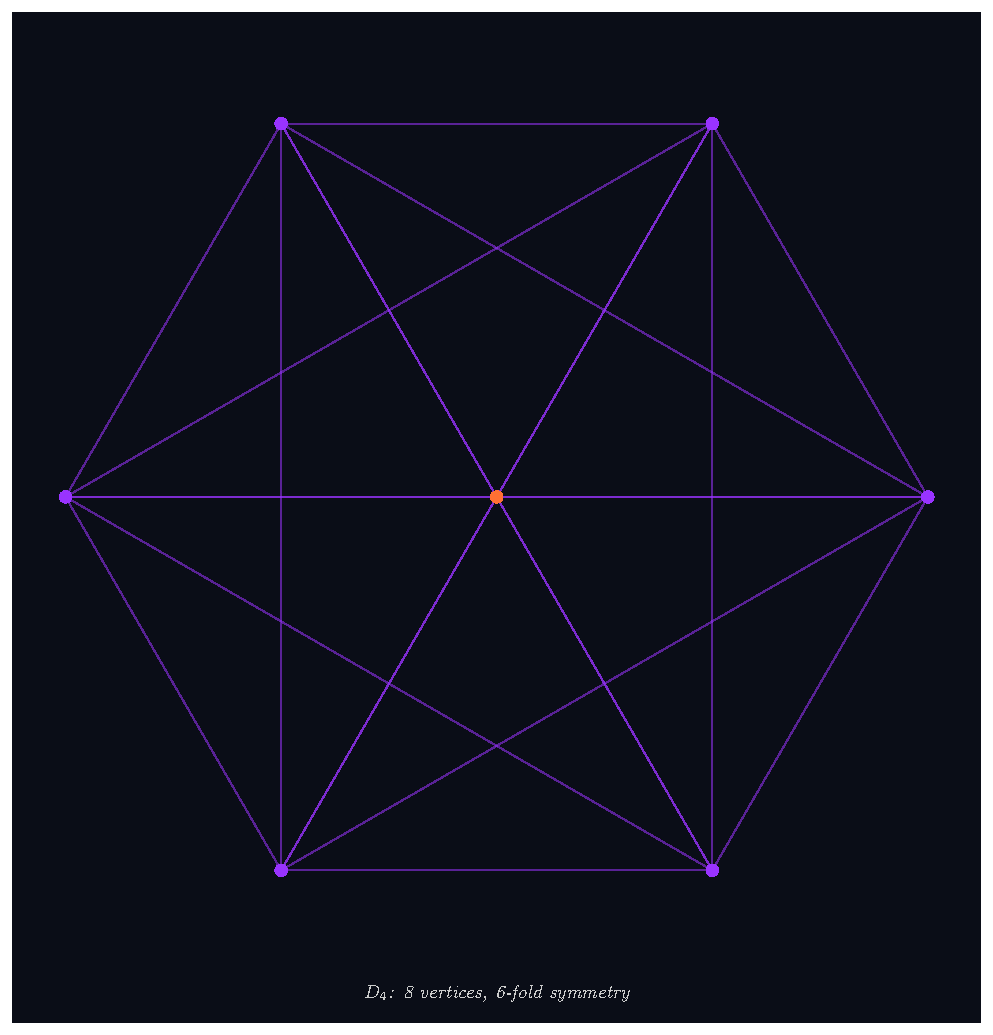
\includegraphics[width=0.38\textwidth]{d4_graph.pdf} &
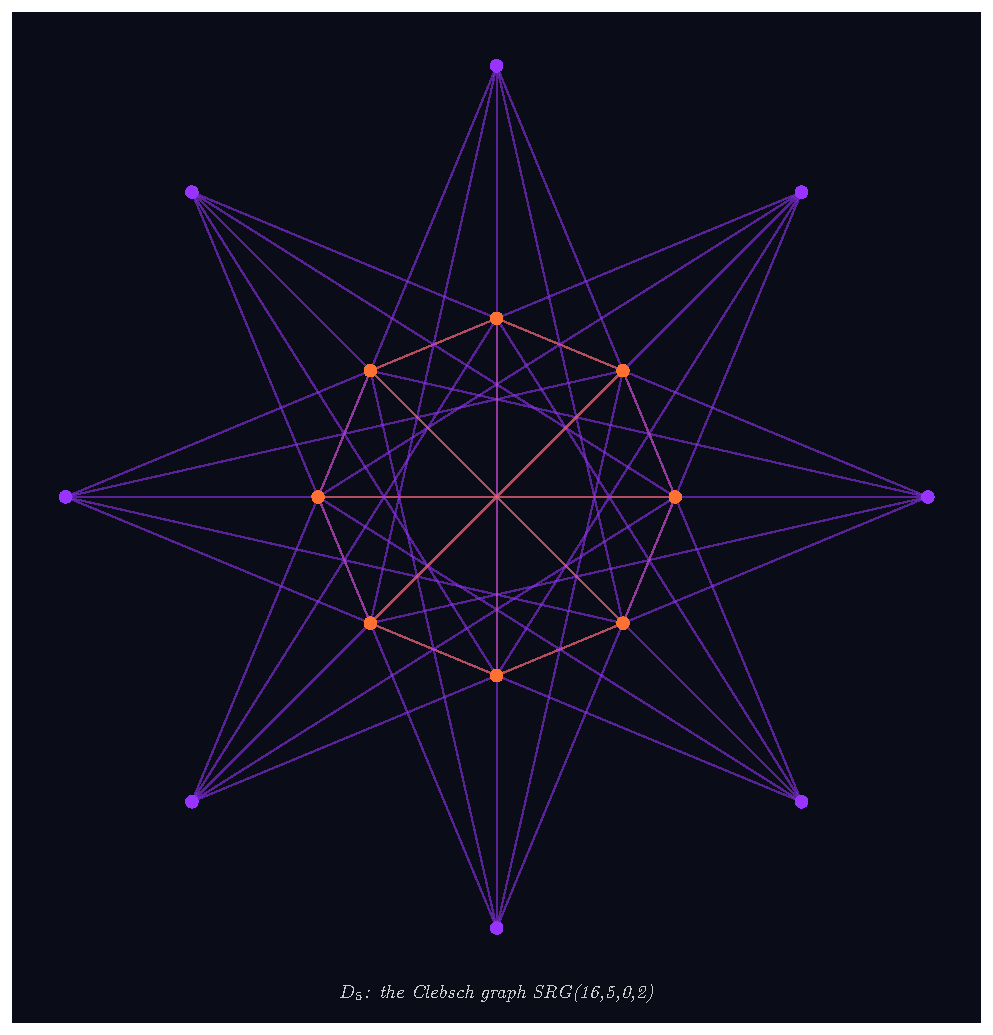
\includegraphics[width=0.38\textwidth]{e5_clebsch.pdf} \\[0.2cm]
\textbf{D4: Triality} & \textbf{D5: The Clebsch} \\
8 vertices, 6-fold & 16 vertices, 8-fold \\[0.6cm]

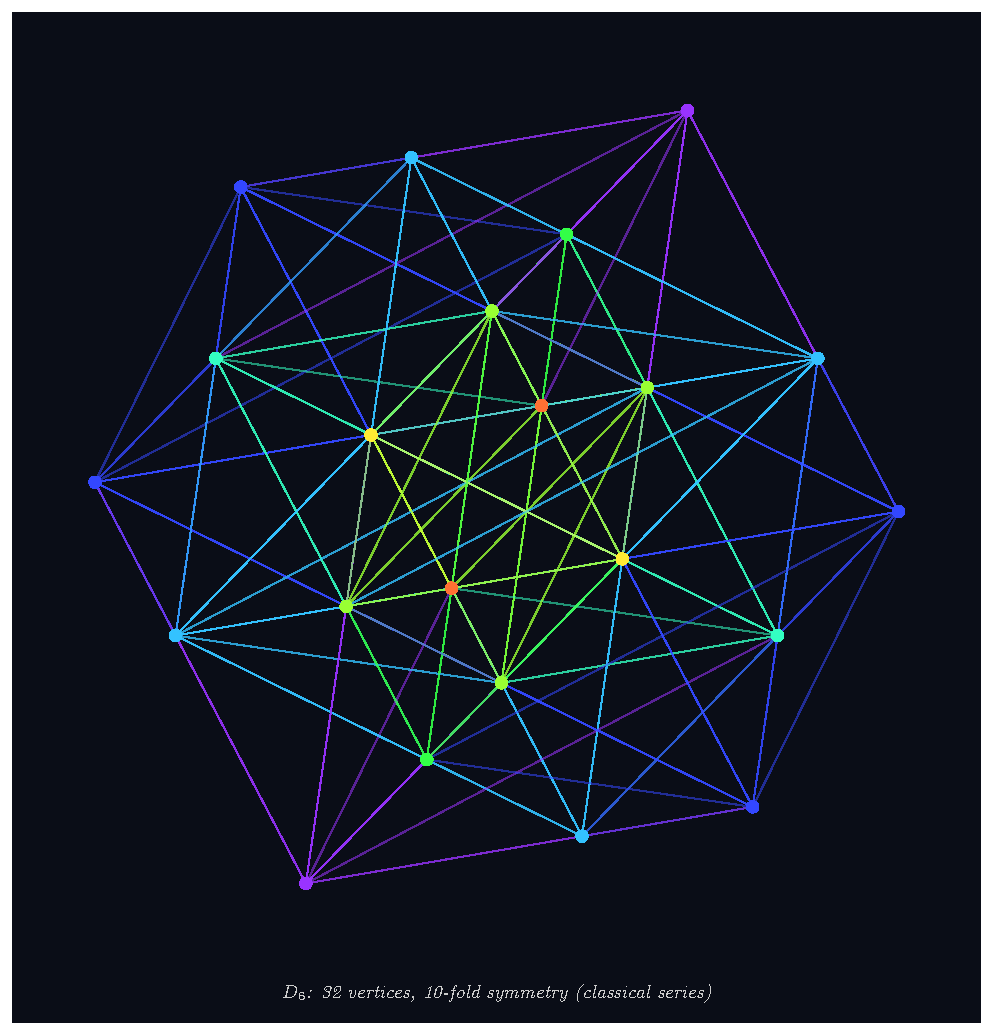
\includegraphics[width=0.38\textwidth]{d6_graph.pdf} &
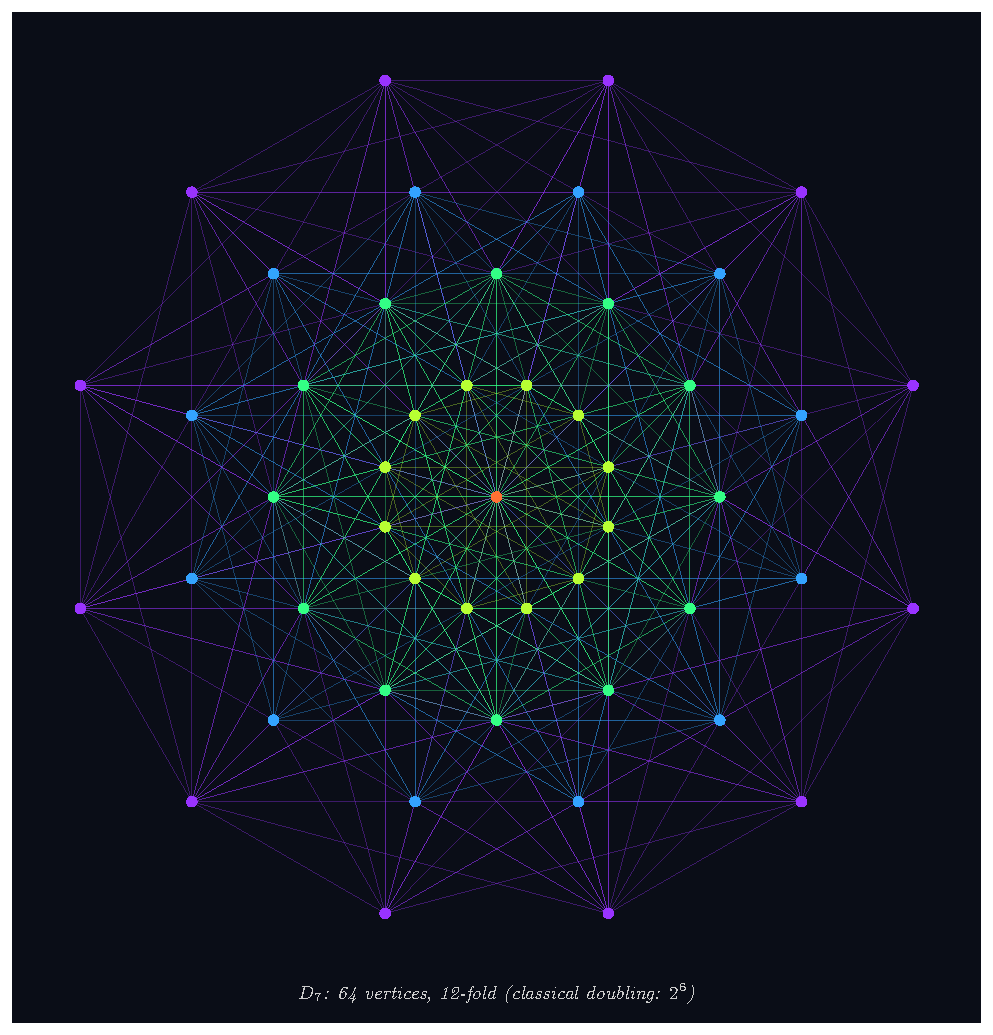
\includegraphics[width=0.38\textwidth]{d7_classical.pdf} \\[0.2cm]
\textbf{D6: The Hexacube} & \textbf{D7: The Heptacube} \\
32 vertices, 10-fold & 64 vertices, 12-fold \\
\end{tabular}
\end{center}

\vspace{0.5cm}

\textit{Pattern: $D_n$ has $2^{n-1}$ vertices, Coxeter number $h = 2n-2$.
The series continues forever: D8, D9, \ldots with predictable doubling.}

\clearpage

%% PAGE 3: THE A-SERIES (SIMPLICES)
\section*{III. The A-Series (Simplices)}

\begin{center}
\begin{tabular}{cc}
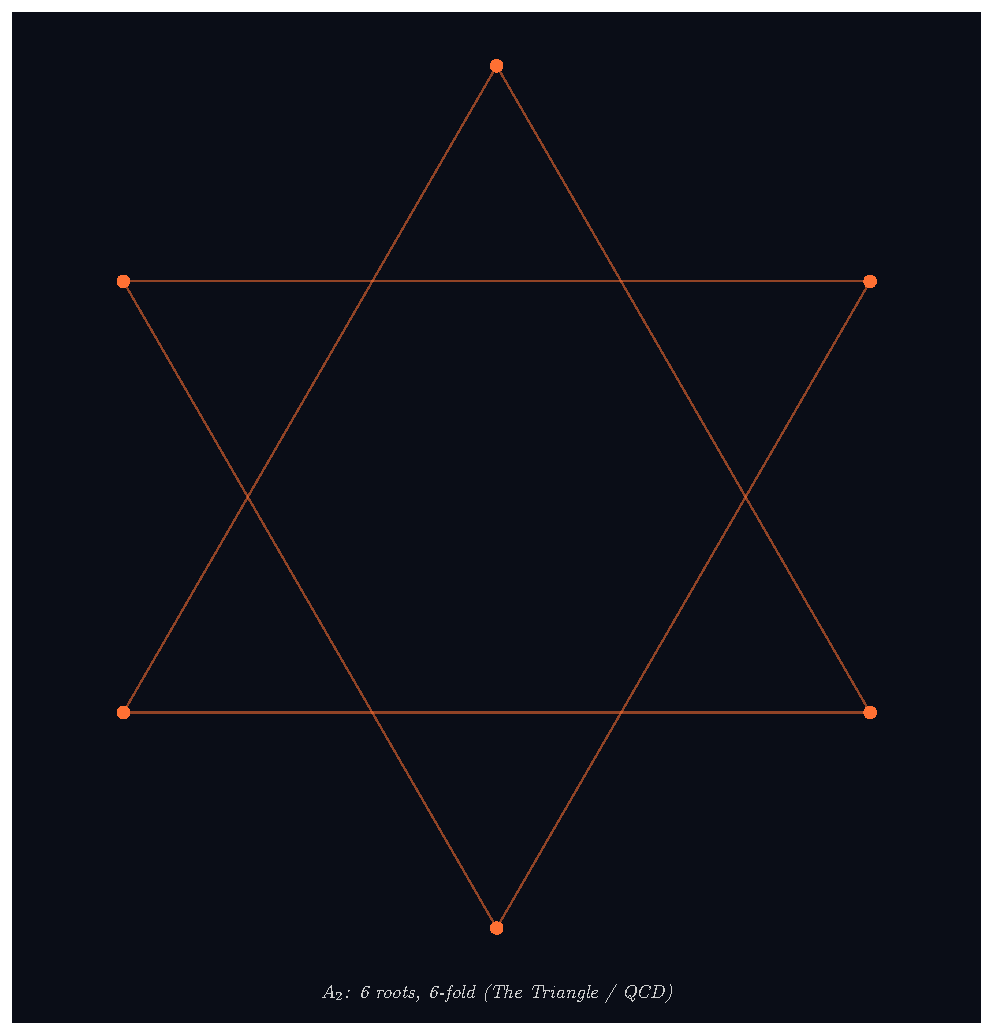
\includegraphics[width=0.38\textwidth]{a2_roots.pdf} &
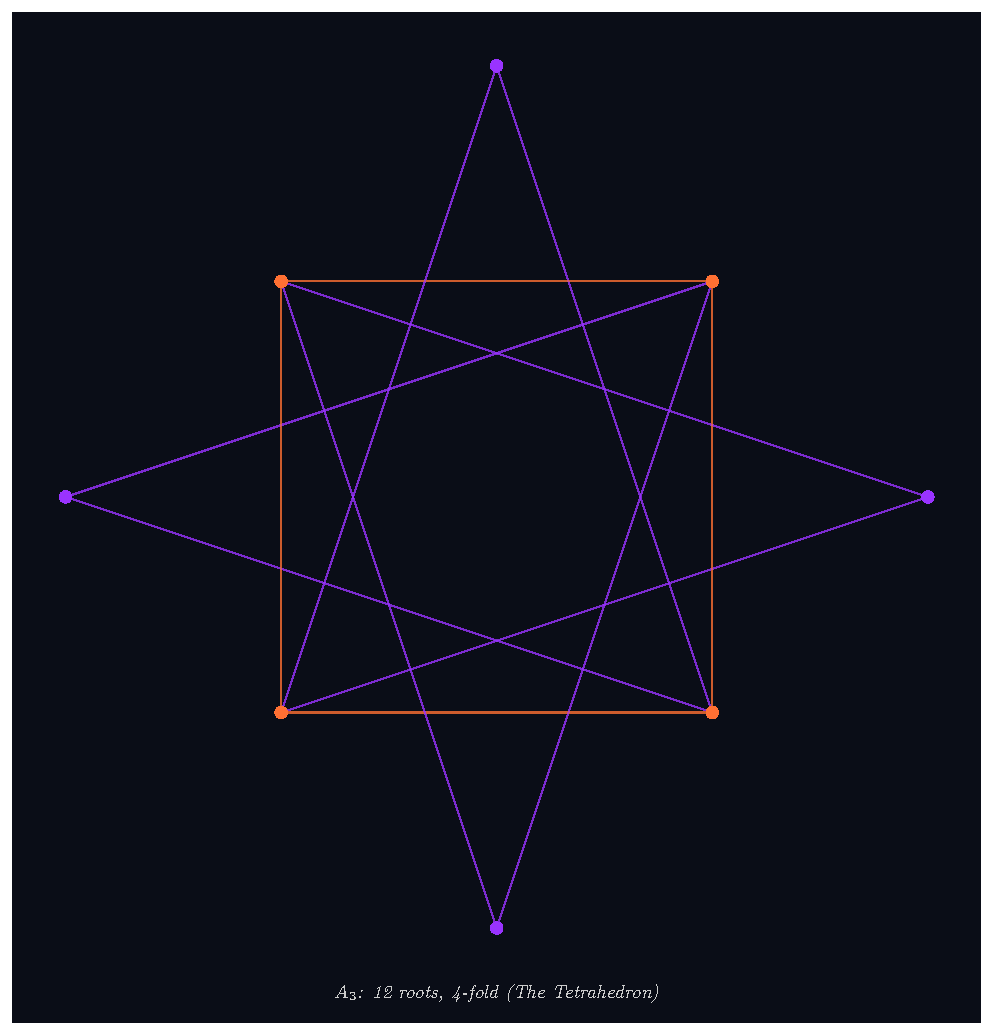
\includegraphics[width=0.38\textwidth]{a3_roots.pdf} \\[0.2cm]
\textbf{A2: The Triangle / QCD} & \textbf{A3: The Tetrahedron} \\
6 roots, 6-fold & 12 roots, 4-fold \\
3 vertices (SU(3)) & 4 vertices (Platonic solid) \\
\end{tabular}
\end{center}

\vspace{1cm}

\textit{Pattern: $A_n$ corresponds to SU($n+1$), with $n+1$ vertices forming an $n$-simplex.
The root system has $(n+1)n$ roots. The series continues: A4 (5-simplex), A5, \ldots}

\vspace{1cm}

\subsection*{The Complete Ladder}

\begin{center}
\begin{tabular}{lcccc}
\hline
\textbf{Type} & \textbf{Vertices} & \textbf{Coxeter $h$} & \textbf{Polytope} & \textbf{Series} \\
\hline
$A_2$ & 3 & 3 & triangle & \\
$A_3$ & 4 & 4 & tetrahedron & Classical \\
$D_4$ & 8 & 6 & 16-cell (triality) & (infinite) \\
$D_5$ & 16 & 8 & demihypercube & \\
$D_6$ & 32 & 10 & demihypercube & \\
$D_7$ & 64 & 12 & demihypercube & \\
\hline
$G_2$ & --- & 6 & hexagon & \\
$F_4$ & --- & 12 & 24-cell & Exceptional \\
$E_6$ & 27 & 12 & $2_{21}$ & (finite) \\
$E_7$ & 56 & 18 & $3_{21}$ & \\
$E_8$ & 240 & 30 & $4_{21}$ & \\
\hline
\end{tabular}
\end{center}

\clearpage

%% PAGE 4: THE COMPARISON
\section*{IV. Why E8 is the Endpoint}

\begin{center}
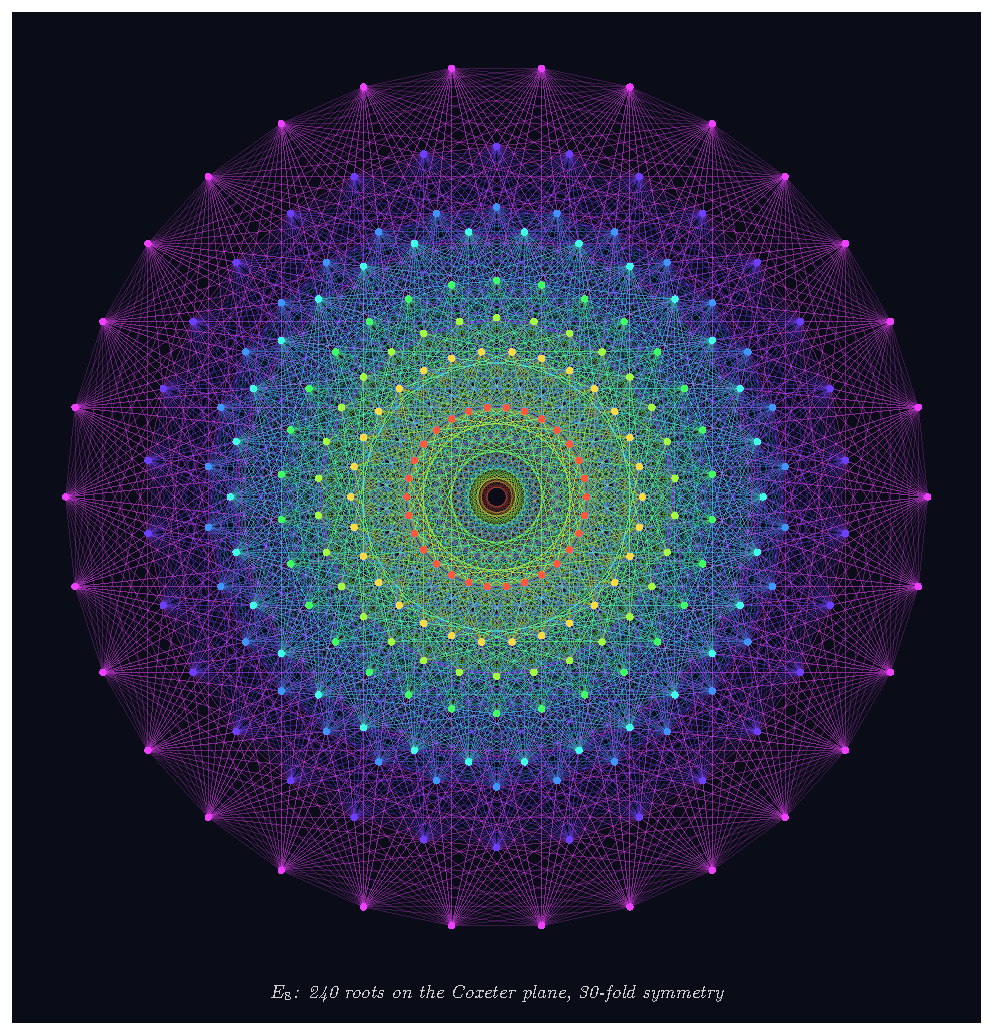
\includegraphics[width=0.42\textwidth]{e8_mandala.pdf}
\hspace{0.5cm}
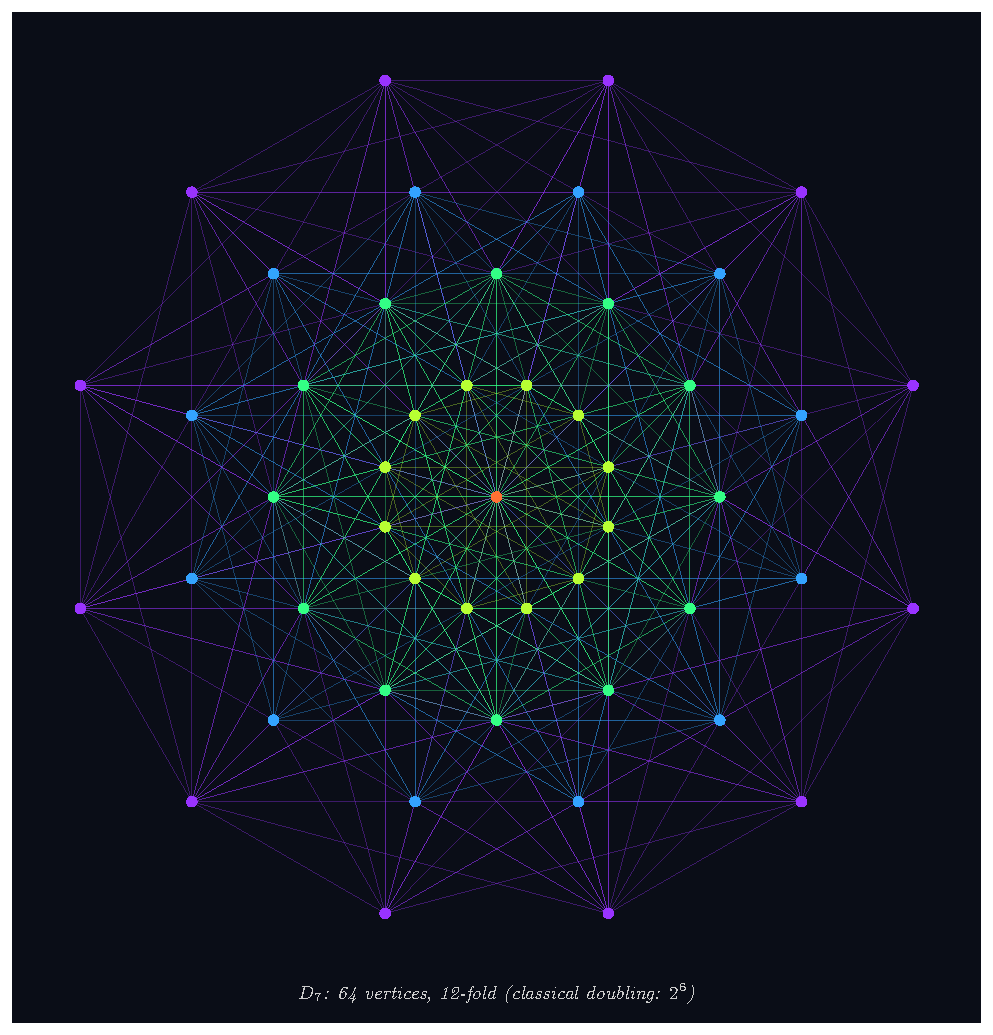
\includegraphics[width=0.42\textwidth]{d7_classical.pdf}

\vspace{0.3cm}
\textbf{E8 (exceptional)} vs \textbf{D7 (classical)}
\end{center}

\vspace{0.5cm}

\subsection*{The Aesthetic Argument}

\textbf{What makes the exceptional series special?}

\begin{itemize}
\item \textbf{Non-doubling vertex counts:} 27, 56, 240 (not powers of 2)
\item \textbf{Irregular symmetry growth:} $12 \to 18 \to 30$ (not arithmetic)
\item \textbf{Numerical magic:} 27 = lines on cubic surface, 56 = 7×8, 240 = kissing number in 8D
\item \textbf{Prime factors:} E8 and E7 have 7 in their group orders; E6 does not
\item \textbf{Perfect interlocking:} $E_6 \subset E_7 \subset E_8$ as nested structures
\end{itemize}

\textbf{Beyond E8:}
\begin{itemize}
\item There is no E9
\item D7 and E6 both have $h=12$, but D7 follows power-of-2 pattern (64 = $2^6$)
\item The polytope $5_{21}$ exists but reverts to classical D-series patterns
\item The exceptional story \textbf{ends at E8 by geometric necessity}
\end{itemize}

\clearpage

%% PAGE 5: THE BESTIARY LIST (PARTIAL)
\section*{V. The Complete Bestiary: 112 Carter Classes}

\small
\begin{multicols}{2}

\subsection*{The Five Exceptional Primes}

\textbf{1. E8} - The Ouroboros / World Serpent\\
\textit{``In my end is my beginning''}

\textbf{2. E7} - The Sacred Cow / Hepta-Mother\\
\textit{``Seven sacred syllables, twice spoken''}

\textbf{3. E6} - The Trinity / Cubic Oracle\\
\textit{``Three times three times three''}

\textbf{4. F4} - The Tesseract Guardian\\
\textit{``Four dimensions, perfectly folded''}

\textbf{5. G2} - The Hexagon / Primal Inchworm\\
\textit{``Six petals of the first flower''}

\subsection*{Exceptional Hybrids}

\textbf{6. E7A1} - The Serpent and the Spinor\\
\textit{``The wyrm coiled around the axis mundi''}

\textbf{7. E6A2} - The Cubic Triangle\\
\textit{``Where form meets force''}

\textbf{8. E6A1\textsuperscript{2}} - The Cubic Twin Spins\\
\textit{``The diamond's double turning''}

\textbf{9. D8} - The Octocube / Classical Shadow\\
\textit{``The shadow cast by the snake''}

\textbf{10. D7A1} - The Heptacube Spin\\
\textit{``The seven-chambered heart, beating''}

\textbf{11. D6A2} - The Hexacube Triangle

\textbf{12. D5A3} - The Pentacube Tetrahedron\\
\textit{``The five-fold hall of four pillars''}

\textbf{13. D4\textsuperscript{2}} - The Twin Trialities\\
\textit{``The mirror shows another mirror''}

\textbf{14. D4A4} - The Tesseract Pentachoron

\textbf{15. A8} - The Ennead / 9-Simplex\\
\textit{``The nine muses in council''}

\textbf{16. A7A1} - The Octad and the Monad\\
\textit{``Eight notes and the silence between''}

\textbf{17. A6A2} - The Heptad Triangle

\textbf{18. A5A2A1} - The Cosmic Dice\\
\textit{``The bones of creation, cast''}

\textbf{19. A4\textsuperscript{2}} - The Twin Pentachorons

\textbf{20. A4A3A1} - The 5-4-2 Chord

\subsection*{Classical Dominance}

\textbf{21-40.} D-series heavy combinations:\\
D8, D7A1, D6A2, D6A1\textsuperscript{2}, D5A3, D5A2A1, D5A1\textsuperscript{3}, D4A4, D4A3A1, D4A2\textsuperscript{2}, D4A2A1\textsuperscript{2}, D4A1\textsuperscript{4}, ...

\subsection*{Simplex Dominance}

\textbf{41-70.} Pure A-series combinations:\\
A8, A7A1, A6A2, A6A1\textsuperscript{2}, A5A3, A5A2A1, A5A1\textsuperscript{3}, A4\textsuperscript{2}, A4A3A1, A4A2\textsuperscript{2}, A4A2A1\textsuperscript{2}, A4A1\textsuperscript{4}, A3\textsuperscript{3}A2, A3\textsuperscript{2}A2\textsuperscript{2}, A3\textsuperscript{2}A1\textsuperscript{2}, A3A2\textsuperscript{2}A1, A3A2A1\textsuperscript{3}, A3A1\textsuperscript{5}, A2\textsuperscript{4}, A2\textsuperscript{3}A1\textsuperscript{2}, A2\textsuperscript{2}A1\textsuperscript{4}, A2A1\textsuperscript{6}, ...

\textbf{63. A1\textsuperscript{8}} - The Octave / Eight-Fold Path\\
\textit{``Eight bells ringing in different towers''}

\subsection*{The Exotics}

\textbf{71-85.} F4 and G2 combinations

\textbf{86-112.} Complex small mixtures

\end{multicols}

\vspace{0.5cm}

\begin{center}
\textit{The complete classification requires 112 conjugacy classes in W(E8),\\
each labeled by its Levi subsystem decomposition.\\
This is Carter's classification (1972).}
\end{center}

\end{document}
